%%\documentclass[twocolumn,notitlepage,10pt]{article}
\usepackage[preprint]{acmconf} 
\usepackage{times}
\renewcommand{\ttdefault}{cmtt}
\usepackage{mathptm}

\usepackage{alltt}
\usepackage{epsfig}
\usepackage{verbatim}
\usepackage{fancybox}

\hyphenation{PowerScope Power-Scope}

\newcommand\unit{\,}

\setlength\abovecaptionskip{0pt}
\setlength\belowcaptionskip{2pt plus 1pt minus 1pt}
\setlength{\floatsep}{6pt plus 5pt minus 2pt}
\setlength{\dblfloatsep}{6pt plus 5pt minus 2pt}
\setlength{\textfloatsep}{6pt plus 10pt minus 3pt}
\setlength{\dbltextfloatsep}{6pt plus 10pt minus 3pt}

%\renewcommand{\topfraction}{0.9}
%\renewcommand{\bottomfraction}{0.9}
%\renewcommand{\textfraction}{0.1}
%\renewcommand{\floatpagefraction}{0.9}

\parskip 3pt plus 2pt minus 2pt    
        
\makeatletter

\renewcommand{\section}{\@startsection
  {section}%
  {1}%
  {0mm}%
  {6pt plus 2pt}%
  {6pt plus 2pt}%
  {\normalfont\Large\bf}}

\renewcommand{\subsection}{\@startsection
  {subsection}%
  {2}%
  {0mm}%
  {4pt plus 2pt}%
  {4pt plus 2pt}%
  {\normalfont\large\bf}}

\renewcommand{\subsubsection}{\@startsection
  {subsubsection}%
  {3}%
  {0mm}%
  {2pt plus 2pt}%
  {2pt plus 2pt}%
  {\normalfont\normalsize\bf}}

\def\maketitle{\par
 \begingroup
   \def\thefootnote{\fnsymbol{footnote}}
   \def\@makefnmark{\hbox
       to 0pt{$^{\@thefnmark}$\hss}}
   \if@twocolumn
     \twocolumn[\@maketitle]
     \else \newpage
     \global\@topnum\z@         % Prevents figures from going at top of page.
%     \@maketitle \fi\thispagestyle{empty}\@thanks
     \@maketitle \fi\@thanks
 \endgroup
 \setcounter{footnote}{0}
 \let\maketitle\relax
 \let\@maketitle\relax
 }



\newenvironment{captiontext}{%
   \begin{center}%
     \begin{minipage}{0.9\linewidth}%
       \renewcommand{\baselinestretch}{0.9}%
         \sffamily\small}%
   {\renewcommand{\baselinestretch}{1.0}%
      \end{minipage}%
        \end{center}}

\newenvironment{smenumerate}%
  { \newcounter{foo_counter}
    \begin{list}{\arabic{foo_counter}}%
     {\usecounter{foo_counter}
      \setlength{\parsep}{0pt}%
      \setlength{\topsep}{0pt}%
      \setlength{\itemsep}{2pt}}}%
  {\end{list}}

\newenvironment{smitemize}%
  {\begin{list}{$\bullet$}%
     {\setlength{\parsep}{0pt}%
      \setlength{\topsep}{0pt}%
      \setlength{\itemsep}{2pt}}}%
  {\end{list}}

\newenvironment{sm1enumerate}%
  { \newcounter{foo_counter}
    \begin{small}\begin{list}{\arabic{foo_counter}}%
     {\usecounter{foo_counter}
      \setlength{\parsep}{0pt}%
      \setlength{\topsep}{0pt}%
      \setlength{\itemsep}{5pt}}}%
  {\end{list}\end{small}}

\newenvironment{sm1itemize}%
  {\begin{small}\begin{list}{$\bullet$}%
     {\setlength{\parsep}{0pt}%
      \setlength{\topsep}{0pt}%
      \setlength{\itemsep}{5pt}}}%
  {\end{list}\end{small}}


\newenvironment{ColVerb}%
	{\VerbatimEnvironment
	\begin{Sbox}\begin{minipage}{73mm}\begin{alltt}}%
	{\end{alltt}\end{minipage}\end{Sbox}
	\setlength{\fboxsep}{3mm}\fbox{\TheSbox}}

\newenvironment{PageVerb}%
	{\VerbatimEnvironment
	\begin{Sbox}\begin{minipage}{158mm}\begin{alltt}}%
	{\end{alltt}\end{minipage}\end{Sbox}
	\setlength{\fboxsep}{3mm}\fbox{\TheSbox}}

\newenvironment{abstracttext}{%
     \begin{minipage}{0.9\linewidth}%
       \renewcommand{\baselinestretch}{0.9}%
         \small}%
      {\renewcommand{\baselinestretch}{1.0}%
     \end{minipage}}


%\makeatletter
\long\def\unmarkedfootnote#1{{\long\def\@makefntext##1{##1}\footnotetext{#1}}}
\makeatother

\documentclass{article}
\usepackage{times}
\usepackage{mathptm}
\usepackage{url,epsfig,graphicx,color}
\usepackage{cite,xspace}

\newcommand{\rw}[1]{{\em #1}}

\title{Diamond Design}
\author{
  Larry Huston
}

\begin{document}

\maketitle


\section{Introduction}
\label{Introduction}

The document provides an overview of the different components 
in the Diamond implementation and how they integrate together.

The Diamond implementation is currently implemented as user
space Linux software.   There are two logical pieces of
software the host code and the active disk code.  Each of these
are built using a set of libraries, many of these libraries are
in common between both implementations.

Many of the different library implementations create their
own thread of control to perform work.  In almost all
cases any communcation between the various components
is asynchronous (message passing).  This allows us
to get maximum concurrency.  This also applies to all
of the communications between the host and the storage devices.


\subsection{Host Implementation}

The host implemenation is a library that is linked against the domain
application.  This library is composed of several other libraries
that do most of the work.  Figure~\ref{fig:hostoverview} shows
the major components of this library.

\begin{figure}[tbp]
\begin{center}
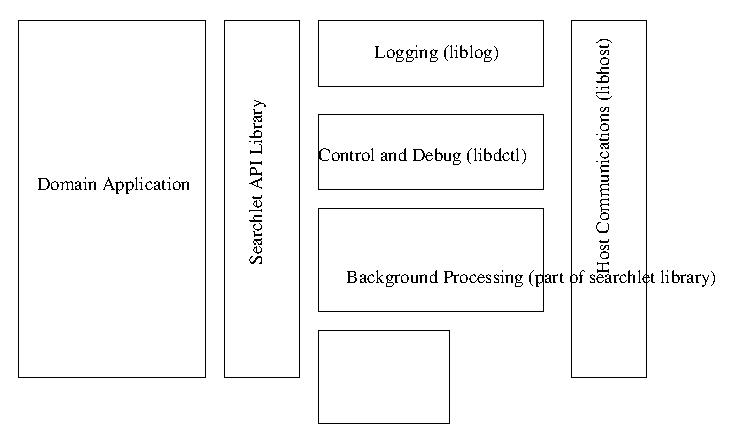
\includegraphics[width=\linewidth]{pics/host_structure}%
\end{center}
\caption{\textbf\{Host Implementation.}
The different components of the host implementation.
XXX fill in.
\label{fig:hostoeverview}
\end{figure}
                                                                                


\subsection{Disk Implementation}



\end{document}
